\section{Uvod}
\hspace{\parindent}Algoritam šišmiša\cite{Yang2010} (BA) metaheuristički je optimizacijski algoritam iz skupine algoritama rojeva čestica. Nadahnut je eholokacijom šišmiša. 

\hspace{\parindent} Šišmiši su sisavci iz roda \textit{Chiroptera} i ujedno jedini sisavci s krilima. Tvore oko 20\% svih vrsta sisavaca.  Dijele su 2 podreda: veliki šišmiši (\textit{Macrochiroptera}) i mali šišmiši (\textit{Microchiroptera}). Iako sve vrste koriste eholokaciju u nekoj mjeri,  šišmiši iz reda malih šišmiša je koriste opsežnije.\cite{netopiri}  Eholokacija kod malih šišmiša oblik je sonara, odašilju vrlo glasan i kratkotrajan zvučni impuls te primaju jeku koju je izazvao odbijajući se od okoline. Služi im za pronalaženje plijena, svojih legla i izbjegavanje prepreka u mraku. 

\hspace{\parindent} Za većinu vrsta impuls traje između 5 i 20 ms i ima konstantnu frekvenciju u intervalu od 25 kHz do 150 kHz. U normalnim uvjetima taj impuls odašilju 10 do 20 puta u sekundi, dok  ga prilikom lova mogu odašiljati i do 200 puta u sekundi. Ispostavlja se da šišmiši imaju izrazitu sposobnost obrade signala. Uz pretpostavku brzine zvuka od 340 m/s, može se odrediti da je valna duljina impulsa između 2mm i 14mm za frekvencijski raspon od 25 kHz do 150 kHz. Intenzitet zvuka može biti do 110 dB, a smanjuje se što je šišmiš bliže plijenu.

\section{Algoritam}
\hspace{\parindent}U samom algoritmu potrebno je idealizirati svojstva eholokacije:
\begin{enumerate}
	\item Svi šišmiši koriste eholokaciju radi određivanja udaljenosti.
        \item Znaju razliku između plijena i prepreka.
	\item i-ti šišmiš leti brzinom $\vec{v_i}$, na položaju $\vec{x_i}$, s frekvencijom $f_i$ i intenzitetom zvuka $A_i$.
 \item Šišmiši namještaju frekvenciju zvučnih impulsa i učestalost odašiljanja $r \in [0,1]$ prema udaljenosti od plijena.
	\item Intenzitet zvuka je u intervalu $[A_{\text{min}}, A_0]$.
 \item Frekvencija je u intervalu $[f_{\text{min}},f_{\text{max}}]$.
\end{enumerate}


Pretpostavlja se da postoji $N$ šišmiša u prostoru dimenzije $n$. U svakoj iteraciji algoritma, svaki šišmiš izvodi 3 radnje:
\begin{enumerate}
    \item Kretanje
    \item Lokalna pretraga
    \item Ažuriranje intenziteta zvuka i učestalosti odašiljanja
\end{enumerate}





\subsection{Kretanje}
\hspace{\parindent}Kretanje je slično kretanju čestica u algoritmu roja čestica. U svakom koraku vektor brzine se usmjeri prema najboljem rješenju i odvije se kretanje šišmiša. Promjena vektora brzine ovisi o frekvenciji. 

Položaj $i$-tog od $N$ šišmiša u koraku $t$ predstavlja $n$-dimenzionalni vektor:
\begin{equation}
	\vec{x_i}^t = (x_{i1}^t, x_{i2}^t, \dots, x_{in}^t)
\end{equation}
Brzinu $i$-tog od $N$ šišmiša u koraku $t$ predstavlja $n$-dimenzionalni vektor:
\begin{equation}
	\vec{v_i}^t = (v_{i1}^t, v_{i2}^t, \dots, v_{in}^t)
\end{equation}
U koraku $t$ računa se nova frekvencija:
\begin{equation}
	f_i = f_{\text{min}} + (f_{\text{max}} - f_{\text{min}})\beta
\end{equation}

gdje je $\beta$ realan broj uzorkovan iz uniformne razdiobe na intervalu $[0,1]$.\\
U koraku $t$ računa se nova brzina:
\begin{equation}
	\vec{v_i}^t = \vec{v_i}^{t-1} + (\vec{x_i}^* - \vec{x_i}^{t-1})f_i
\end{equation}

gdje je $\vec{x_i}^*$ položaj šišmiša s najvećom vrijednošću ciljne funkcije u koraku $t-1$.\\
U koraku $t$ računa se novi položaj:
\begin{equation}
	\vec{x_i}^t = \vec{x_i}^{t-1} + \vec{v_i}^{t}
\end{equation}

\subsection{Lokalna pretraga}
\hspace{\parindent}Nakon što su svi šišmiši završili s kretanjem, pokreće se lokalna pretraga za svakog šišmiša. Lokalna je pretraga nasumična. Položaj šišmiša se ažurira na sljedeći način:
\begin{equation}
	\vec{x}_\text{novi} = \vec{x}_\text{stari} + \varepsilon A^t
\end{equation}
gdje je $\varepsilon$ slučajan broj iz intervala $[-1, 1]$, a $A^t$ je srednja vrijednost intenziteta zvuka svih šišmiša.


\subsection{Intenzitet zvuka i učestalost odašiljanja}
\hspace{\parindent}Ako je iznos funkcije cilja u novom položaju šišmiša bolji od onog u prethodnom, novi se  položaj prihvaća te se ažuriraju intenzitet zvuka i učestalost odašiljanja.
U koraku $t$ računa se novi intenzitet zvuka:
\begin{equation}
	A_i^{t} = \alpha A_i^{t - 1}
\end{equation}
U koraku $t$ računa se nova učestalost odašiljanja:
\begin{equation}
	r_i^{t} = r_i^{0}[1 - e^{-\gamma(t-1)}]
\end{equation}
Konstante $\gamma$ i $\alpha$ su parametri algoritma. Oni određuju brzinu konvergencije. Za svaki $ 0 < \alpha < 1$ i $\gamma > 0$, vrijedi:
\begin{equation}
	\lim_{t \to \infty} A_i^{t} = 0
\end{equation}
\begin{equation}
	\lim_{t \to \infty} r_i^{t} = r_i^{0}
\end{equation}
Za $r_i = 1$ i $A_i = 0$, algoritam degradira u obični algoritam roja čestica.






\subsection{Pseudokod}

\begin{algorithm}[H]
	\begin{algorithmic}[1]
		\Function{BA}{obj(x), n, N, fmin, fmax, Amin, A0, maxIter, $\alpha$, $\gamma$}
		
\State x = \Call{InitX}{n, d}

\State v = \Call{InitV}{n, d}

\State f = \Call{InitF}{fmin, fmax}
  
\State A = \Call{InitA}{Amin, A0}
  
  \State r0 = r = \Call{InitR}{0,1} \Comment{Inicijalizacija struktura podataka}

  
  \For{iter = 1 to maxIter}
		\For{i = 1 to N} 
  
                
                \State b = \Call{UniformDist}{0, 1}
                \State f[i] = fmin + (fmax - fmin)*b
                \State v'[i] = v[i] + (x* - x[i]) * f[i]
                \State x'[i] = x[i] + v[i] \Comment{Kretanje šišmiša}

                \State rand = \Call{UniformDist}{0, 1}
                \If{rand > r[i]}
                \State x'[i] = x* + \Call{NormalDistVec}{n, 0, 1}
                \EndIf
                \State e = \Call{UniformDistVec}{n, -1, 1}
                \State Amean = \Call{Mean}{A} 
                \State x'[i] = x'[i] + Amean*e \Comment{Lokalna pretraga}
                \State rand = \Call{UniformDist}{0, 1}
                \If{rand < A[i] AND obj(x'[i]) < obj(x[i])}
                    \State x[i] = x'[i] \Comment{Prihvat novog rješenja}
                    \State v[i] = v'[i]
                    \State A[i] = $\alpha$ * A[i]
                    \State r[i] = r0[i] * (1 - e**(-$\gamma$ * iter))
                \EndIf
                \EndFor
		\State x* = \Call{MaxArg}{obj(x)}
		\EndFor
		\State \Return x*	
		\EndFunction
	\end{algorithmic}
	\caption{Algoritam šišmiša}
\end{algorithm}







\section{Programsko ostvarenje}
\subsection{Primjer funkcije za minimizaciju}
Neka se minimizira $n$-dimenzionalna funkcija:
\begin{equation}
    f(\vec{x}) = \sum_{i = 1}^{n}x_i^2 + 25\sum_{i = 1}^{n}\sin^2{x_i} \label{eq:fx}
\end{equation}



\begin{figure}[H]
	\centering
	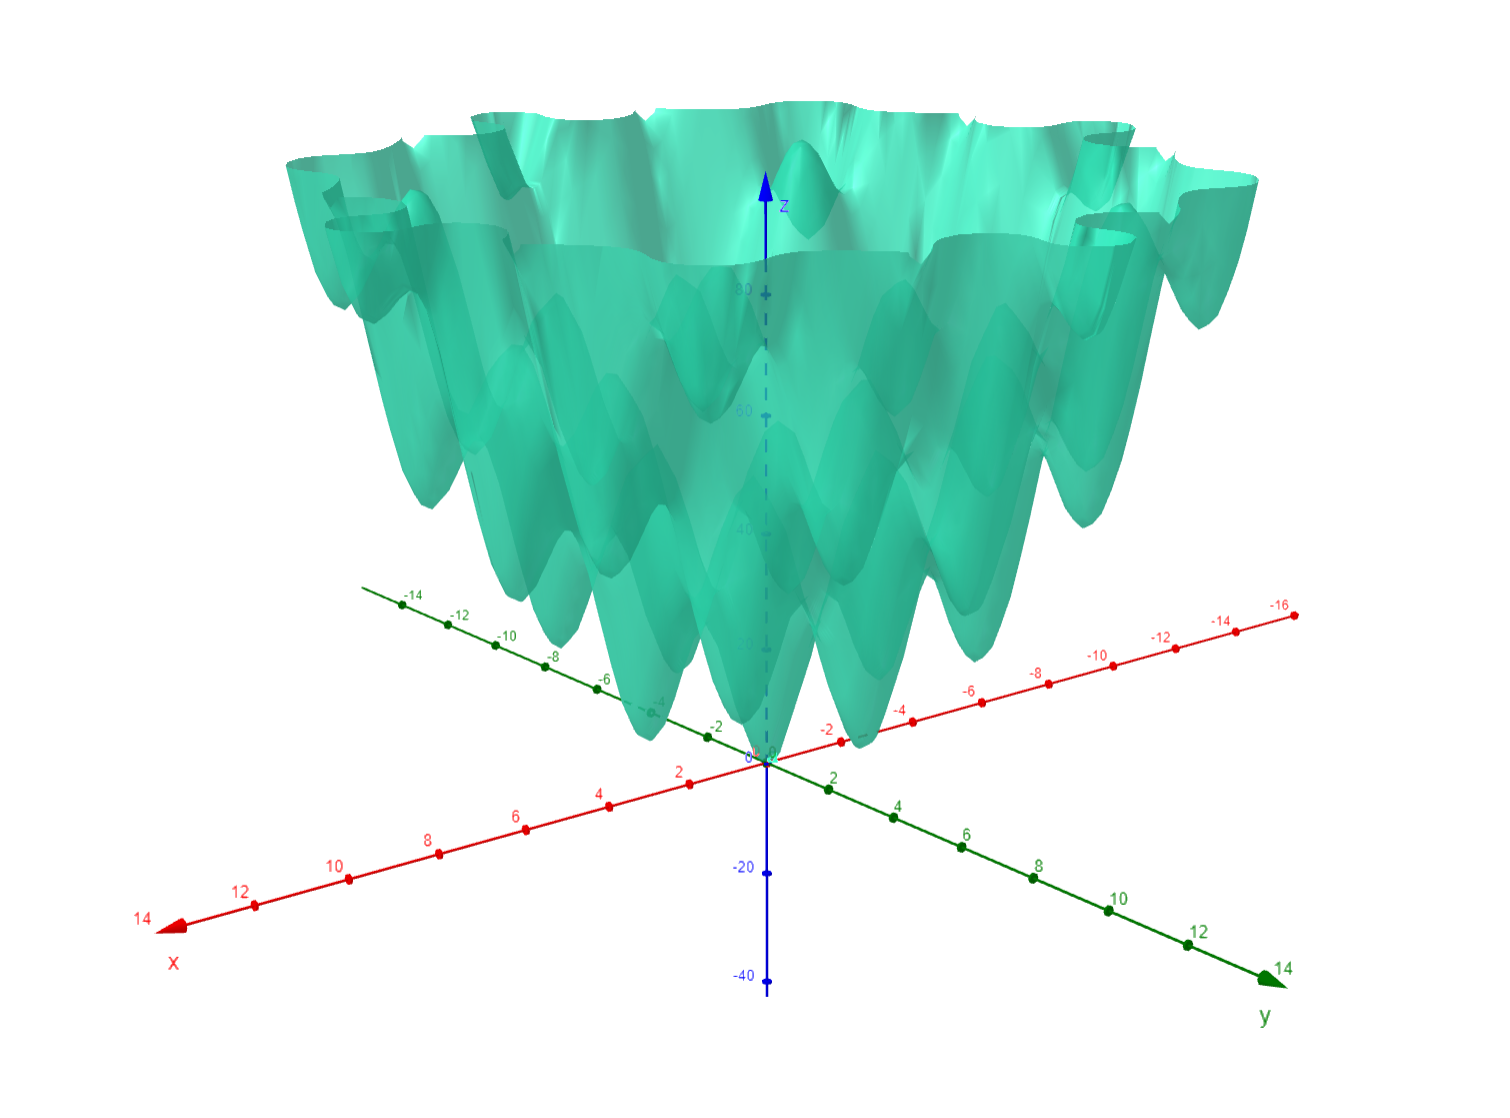
\includegraphics[width=14cm]{eggcrate_func.png}
	\caption{Graf funkcije $f(\vec{x})$ za $n = 2$} 
\end{figure}

Funkcija ima minimum u točki $\vec{0}$ i on iznosi $f(\vec{0}) = 0$. 


\subsection{Programsko ostvarenje MEALPY} \label{MP:Bat}
\hspace{\parindent}Algoritam šišmiša i mnogi drugi metaheuristički algoritmi programski su ostvareni u sklopu knjižnice programa otvorenog koda MEALPY\cite{van2023mealpy} programskog jezika Python. Knjižnica se može preuzeti naredbom konzole:

\begin{figure}[H]
	\begin{framed}
		\begin{footnotesize}
			\begin{verbatim}
		> pip install mealpy\end{verbatim}
		\end{footnotesize}
	\end{framed}
	\captionof{Kod}{Naredba konzole za preuzimanje knjižnice MEALPY}
\end{figure}

\hspace{\parindent}Prethodno opisani problem funkcije \eqref{eq:fx} s $n = 10$ definira se u programu kao rječnik i pokreće se algoritam šišmiša s 1000 iteracija, brojem šišmiša $N = 50$,  $\alpha = \gamma = 0.9$, $[A_{\text{min}}, A_0] = [1, 2]$,  $[f_{\text{min}}, f_{\text{max}}] = [-10, 10]$. U razredu \verb|BA| postoji više različitih inačica algoritma, najsličniji opisanom je \verb|AdaptiveBA|, stoga je on korišten u primjeru.

\begin{figure}[H]
	\begin{framed}
		\begin{footnotesize}
			\begin{verbatim}
import numpy as np
from mealpy import FloatVar, BA
from numpy import pi as PI

n = 10

def objective_function(solution):
    return np.sum(solution**2) + 25*np.sum(np.sin(solution)**2)

problem = {
    "obj_func": objective_function,
    "bounds": FloatVar(lb=(-2*PI,)*n, ub=(2*PI,)*n),
    "minmax": "min",
}


model = BA.AdaptiveBA(epoch=1000, pop_size=50, 
                      loudness_min = 1.0, loudness_max = 2.0,
                      pf_min = -10., pf_max = 10.)

g_best = model.solve(problem)

print("Solution:", g_best.solution)
print("Fitness:", g_best.target.fitness)
			\end{verbatim}
		\end{footnotesize}
	\end{framed}
	\captionof{Kod}{Pokretanje optimizacije vlastite funkcije}
\end{figure}

\begin{figure}[H]
	\begin{framed}
		\begin{footnotesize}
			\begin{verbatim}
Solution: [-0.07566663 -2.81959093 ...  0.12792114]
Fitness: 106.61031296676825
			\end{verbatim}
		\end{footnotesize}
	\end{framed}
	\captionof{Ispis}{Ispis primjera}
\end{figure}





\section{Algoritam šišmiša u primjeni}

\subsection{Modeliranje dinamike bioloških sustava}
\hspace{\parindent}Algoritam šišmiša korišten je za prilagodljiv odabir vrijednosti parametara modela za rekonstrukciju dinamike bioloških sustava.\cite{lin2012} Uspješnost metode je pokazana na primjeru procjene parametara dinamike endocitoze.



\subsection{Procjena položaja ljudskog tijela}
\hspace{\parindent} Praćenje položaja ljudskoj tijela iz snimaka u laboratorijskim uvjetima postavljeno je kao 31-dimenzionalni optimizacijski problem.\cite{akhtar2012} Pokazano je da algoritam šišmiša radi bolje od drugih srodnih algoritama (poput algoritma roja čestica.)



\subsection{Grupiranje}
\hspace{\parindent} Razvijen je algoritam grupiranja temeljen na algoritmu K-sredina i algoritmu šišmiša.\cite{komarasamy2012} Algoritam ne zahtijeva definiranje hiperparametra K, nego sredine pronalazi korištenjem algoritma šišmiša. Prednost je ubrzanje brzine konvergencije algoritma šišmiša i smanjivanje ovisnosti algoritma K-sredina o početno odabranim sredinama.

\subsection{Problem ekonomske raspodjele opterećenja}
\hspace{\parindent} U problemu ekonomske raspodjele opterećenja, cilj je zadovoljiti potrebe za energijom uz minimalne financijske troškove. Optimizacija termalne elektrane provedena je algoritmom šišmiša uz rezultate bolje od rezultata drugih srodnih algoritama.\cite{biswal2013}

\subsection{Podudaranje slika}
\hspace{\parindent} Problem podudaranja slika u računalnom vidu je poistovjećivanje slika istih objekata slikanih u različitim uvjetima.\cite{zhangjia2012} Algoritam šišmiša, uz dodatak mutacija, korišten je za rješavanje ovog problema. Pokazano je da je takav algoritam na ovom problemu učinkovitiji od običnog algoritma šišmiša.

\subsection{Odabir značajki}
\hspace{\parindent} Binarna inačica algoritma šišmiša korištena je za odabir optimalnog podskupa značajki.\cite{6382769} Pristup spaja istraživačku moć šišmiša i brzinu klasifikatora \textit{Optimum-Path Forest} za maksimizaciju točnosti na skupu za provjeru. Pokusima je utvrđeno da takav pristup ima bolje performanse od drugih poznatih algoritama.

\subsection{Optimizacija sustava rezervoara}
\hspace{\parindent} Algoritam šišmiša upotrebljen je za optimizaciju rezervoarskog sustava Karoun-4 u Iranu.\cite{doi:10.1061/(ASCE)WR.1943-5452.0000498} Algoritam je bio učinkovitiji od linearnog programiranja, nelinearnog programiranja i genetskog algoritma. 

\subsection{Online učenje unaprijednih neuronskih mreža}
\hspace{\parindent} Online učenje slojeva unaprijednih neuronskih mreža provedeno je algoritmima: BA, GA i PSO.\cite{khankoffka2012} Usporednom analizom bilo je vidljivo da algoritam šišmiša ima bolje performanse od ostalih.